\documentclass[11pt]{article}
\usepackage{latexsym}
\usepackage{amsmath}
\usepackage{amssymb}
\usepackage{amsthm}
\usepackage{epsfig}
\usepackage[tight]{subfigure}
\usepackage{todonotes} % for comments
\usepackage{float}

\usepackage{amsmath,amssymb}
\usepackage{scrextend}

\DeclareMathOperator*{\minimize}{min}
\DeclareMathOperator*{\maximize}{max}

\usepackage{algorithm}
 %on linux you may need to run sudo apt-get install texlive-full to install algorithm.sys
\usepackage{algorithmic}

\usepackage{verbatim}

\newcommand{\handout}[5]{
  \noindent
  \begin{center}
  \framebox{
    \vbox{
      \hbox to 5.78in { {#1} \hfill #2 }
      \vspace{4mm}
      \hbox to 5.78in { {\Large \hfill #5  \hfill} }
      \vspace{2mm}
      \hbox to 5.78in { {\em #3 \hfill #4} }
    }
  }
  \end{center}
  \vspace*{4mm}
}

\newcommand{\lecture}[5]{\handout{#1}{#2}{#3}{#4}{#5}}
\newcommand{\collision}[0]{\mathrm{collision}}
\newcommand{\nocollision}[0]{\overline{\collision}}

\newcommand*{\QED}{\hfill\ensuremath{\square}}

\newtheorem{theorem}{Theorem}
\newtheorem{corollary}[theorem]{Corollary}
\newtheorem{lemma}[theorem]{Lemma}
\newtheorem{observation}[theorem]{Observation}
\newtheorem{proposition}[theorem]{Proposition}
\newtheorem{definition}[theorem]{Definition}
\newtheorem{claim}[theorem]{Claim}
\newtheorem{fact}[theorem]{Fact}
\newtheorem{assumption}[theorem]{Assumption}
\newtheorem{note}[theorem]{Note}

% 1-inch margins, from fullpage.sty by H.Partl, Version 2, Dec. 15, 1988.
\topmargin 0pt
\advance \topmargin by -\headheight
\advance \topmargin by -\headsep
\textheight 8.9in
\oddsidemargin 0pt
\evensidemargin \oddsidemargin
\marginparwidth 0.5in
\textwidth 6.5in

\parindent 0in
\parskip 1.5ex
%\renewcommand{\baselinestretch}{1.25}

\begin{document}

\lecture{Statistical Techniques in Robotics (16-831, S22)}{Lecture \#02
  (Monday, January 24)}{Lecturer: Kris Kitani}{Scribes: Grace Brueggman, Kevin Gmelin}{Online Learning and Prediction with Expert Advice}

\section{Review}
In the last lecture, on the topic of Robot Learning Problems, we discovered there are a vast number of learning algorithms. We also learned there are three major categories of feedback from learning algorithms. These categories are (1) Exhaustive versus Sampled Feedback, (2) Instructive versus Evaluative Feedback, and (3) One-shot versus Sequence Feedback. In the next three subsections, we will define each of these categories and provide examples of algorithms that are classified as such. Understanding these categories helps to frame the context of this course, which focuses on learning from evaluative feedback, and where the upcoming content falls in the bigger picture of algorithms that are outside of the scope for the semester. On a smaller scale, it grounds us for this topic on PWEA, or Prediction with Expert Advice.

%This section serves as a review of the previous lecture and any other context required to frame the content of the current lecture. 

%You may format the scribes in any way you like, aside from changing font style, size and page format. Please use subsections and paragraphs to increase the readability of your notes.

%Length requirement 1-2 pages.
\subsection{Exhaustive \& Sampled Feedback} 
This distinction of feedback deals with the question: \emph{Does your learner have access to all of the data?} Examples of algorithms that are classified as exhaustive or sampled can be viewed in the Appendix at Table \ref{tab:exh_samp_ex}.

\definition{\normalfont\textbf{Exhaustive Feedback} is the situation where the learner is exposed to all possible situations.} 

\definition{\normalfont\textbf{Sampled Feedback} is the situation where the learner only has access to a sub-set of the possible situations.} 
\normalfont 


\subsection{Instructive \& Evaluative Feedback} 
This distinction of feedback deals with the question: \emph{What kind of feedback do we get from the environment?} Examples of algorithms that are classified as instructive or evaluative can be viewed in the Appendix at Table  \ref{tab:ins_ev_ex}.

\definition{\normalfont\textbf{Instructive Feedback} provides the learner feedback on all possible actions.} 

\definition{\normalfont\textbf{Evaluative Feedback} provides the learner feedback for the chosen action with no mention how the alternative actions would have resulted.}
\normalfont 

\subsection{One-shot \& Sequence Feedback} 
This distinction of feedback deals with the question: \emph{Is the data generation affected by the previous action?} Examples of algorithms that are classified as one-shot or sequence can be viewed in the Appendix at Table \ref{tab:one_seq_ex}.

\definition{\normalfont\textbf{One-shot Feedback} is an isolated event where the outcome of the current action does not affect the next one.}

\definition{\normalfont\textbf{Sequential Feedback} is the situation where the outcome of the current action affects future actions and outcomes.}

\normalfont 





\section{Summary}
\subsection{Online Learning}
\normalfont
In regular supervised learning, there is a training stage where the agent learns the parameters of a model, followed by the test stage where the agent uses its learned model to make predictions. Thus, in supervised learning, the training and test stages are separated. When the training and test stages can't be separated, online learning is used. This is a different type of learning algorithm where the learning is interleaved with execution. 

At each time step, the agent receives some observations. From these observations and the agent's learned models, the agent has to make a prediction. After making a prediction, the agent receives the true outcome. The goal of online learning is to minimize the error between the prediction and true outcome, which is formally encapsulated as regret. This process of online learning is shown below in Figure \ref{fig:online_learning}. 

\begin{figure}[H]
    \centering
    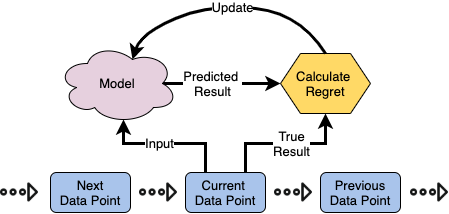
\includegraphics[width=0.7\linewidth]{figures/online learning.png}
    \caption{Online-Learning Flowchart}
    \label{fig:online_learning}
\end{figure}

Unlike supervised learning algorithms, where separate training and test stages require an assumption of a stationary data distribution, online learning algorithms can adapt on-the-fly and can thus work with stochastic, deterministic, and adversarial distributions. 

\definition{\normalfont\textbf{Stochastic Distribution} is when the data has randomness infused and values have a probabilistic nature. It is the opposite of deterministic.}
\normalfont 

An example of stochastic distributed data is a sequence of dice rolls.

\definition{\normalfont\textbf{Deterministic Distribution} is when there is enough information to predict a result with absolute certainty. It is the opposite of stochastic.} 
\normalfont 

An example of deterministic distributed data is a look-up table.

\definition{\normalfont\textbf{Adversarial Distribution} is when the data is generated to specifically break the model.} 
\normalfont 

An example of adversarial distributed data is fast gradient sign \cite{adversarial_ex}.

Online learning can also work with stationary data distributions, but supervised learning algorithms are likely a more appropriate choice for such a data set. Because the online learning model incrementally adapts as it collects more inputs and attempts to minimize regret, duplicate data points previously seen can appear again at later time steps and achieve different results. 

In online learning, the feedback may be either exhaustive or sampled. Furthermore, the feedback may be either instructive or evaluative. However, typically the feedback is one-shot since it is assumed to be not correlated with past feedback and actions. 

Online learning algorithms are useful in cases where:
\begin{itemize}
  \item The feedback is incremental such that learning needs to be interleaved with execution
  \item The training data is too large to process at once
  \item The data distribution changes and the agent needs to adapt
\end{itemize}

Types of online learning algorithms include: 
\begin{itemize}
  \item Prediction with Expert Advice
  \item Bandit
  \item Contextual Bandit
  \item Online Convex Optimization
\end{itemize}

\subsection{Prediction with Expert Advice}
One subset of online learning algorithms is prediction with expert advice (PWEA). The feedback for this set of algorithms is:

\begin{itemize}
    \item One-Shot: We assume the sequence of data is not correlated
    \item Instructive: We receive feedback not only on the chosen action but also on all alternative actions
    \item Exhaustive: Both the action and state spaces are finite and so the learner can be exposed to all possible situations
\end{itemize}

To introduce the topic, let us propose an example modified from How to Use Expert Advice \cite{pwea}:

\begin{addmargin}[2em]{2em}% 2em left, 2em right
Say a learner is trying to predict the weather today, at time ${t = 1}$, where either it will snow, indicated as a 1, or it will not snow, indicated as a 0. Prior to the learner making its prediction, it can consider the predictions of a finite group of local weathermen $\mathcal{E} = \{\mathcal{E}_1, ..., \mathcal{E}_E \}$, here acting as the E experts, where each expert has made a binary prediction $ \textbf{x}^{(1)} \in \{0, 1\}$ about whether it will snow or not. The learner can then make a prediction $ {\hat{y}^{(1)}} \in \{0, 1\}$, where the method of coming to that choice is dependent on the specific algorithm within PWEA utilized. 

By the end of the day, it will have either snowed or not snowed, and the learner will have feedback on not only if the learner predicted correctly, but also feedback for if each of the experts predicted correctly. The next day, where ${t = 2}$, rather than considering all of the experts $ \in \mathcal{E} $, the learner will only consider some of the experts' predictions, choosing the subset of those experts who predicted correctly the day before. This continues day after day, ${t = 3, 4, ..., N}$, with the learner only considering the advice from the experts with a track history of correctly predicting the weather, based on the assumption that this will lead to a better chance of correct weather predictions by the learner.
\end{addmargin}

The essential goal of prediction with expert advice problems is to perform as well as the best prediction strategy, or expert, resulting in a minimized regret \cite{ol_lecture}. 

\definition{\normalfont\textbf{Regret} is the difference between the losses of the learner and the losses of the best expert.} 

\definition{\normalfont\textbf{Loss} is the difference between the predicted result and the true result.} 
\normalfont 

In PWEA problems with E experts, the expert advice at trial t can be represented as an E-dimensional vector: $\textbf{x}^{(t)}$. The advice of the e-th expert is $\textbf{x}^{(t)}_e \in \{0, 1\}$. The set of possible observations is the instance domain, which is represented by $\mathcal{X}$. 

The prediction made by the learner at trial t is specified by $\hat{y}^{(t)} \in \{0, 1\}$. The outcome of trial t is specified by $y^{(t)} \in \{0, 1\}$. The set of all possible outcomes is the target domain, which is represented by $\mathcal{Y}$.

The goal of a prediction with expert advice algorithm such as the greedy algorithm is to find a "good" hypothesis. Here, the notion of good is formalized by the concept of minimizing regret. A hypothesis h is a mapping from the instance domain to the target domain. The set of all possible hypotheses is called the hypothesis class, and it is represented by $\mathcal{H}$.

\subsection{Greedy (Consistent) Algorithm }
\normalfont
One prediction with expert advice algorithm is the greedy algorithm, the pseudocode for which is shown below in Algorithm \ref{algo:greedy}. 

\begin{algorithm}[H]
\caption{Greedy Algorithm}
\label{algo:greedy}
\begin{algorithmic}[1]
\STATE $\textbf{V}^{(1)} = \mathcal{H}$ \hfill $\triangleright$ Version space initially stores all hypotheses
\FOR{$t=1,\;\cdots,\;T$}
\STATE \textsc{Receive} ($\textbf{x}^{(t)}$) \hfill $\triangleright$ Receive expert advice
\STATE $h = \textsc{FirstElement}(\textbf{V}^{(t)})$ \hfill $\triangleright$ Greedy selection
\STATE $\hat{y}^{(t)} = h(\textbf{x}^{(t)})$ \hfill $\triangleright$ Prediction
\STATE \textsc{Receive} ($y^{(t)}$) \hfill $\triangleright$ Receive true outcome
\STATE $\textbf{V}^{(t+1)}) = \{h \in\ \textbf{V}^{(t)} : h(\textbf{x}^{(t)}) = y^{(t)}\}$ \hfill $\triangleright$ Update by keeping only consistent hypotheses

\ENDFOR
\end{algorithmic}
\end{algorithm}

In the greedy algorithm, we maintain a set, called the version space, of hypotheses (maps from the instance domain to the target domain) that have been consistent with every outcome received so far. A hypothesis is consistent if, for every time step, it correctly maps the expert advice at that time step to the true outcome. At each time step, the greedy algorithm first receives expert advice. In order to make a prediction, it selects the first hypothesis from its version space and uses this hypothesis to map the expert advice to a prediction. It then receives the true outcome and it removes all hypotheses from the version space that are inconsistent with this true outcome. 

To expand the previous example of general PWEA to predict the weather, consider the following, a more concrete example in regard to predicting the weather with the Greedy Algorithm:

\begin{addmargin}[2em]{2em}% 2em left, 2em right
There are 5 local weathermen $\mathcal{E} = \{\mathcal{E}_1, \mathcal{E}_2, \mathcal{E}_3, \mathcal{E}_4, \mathcal{E}_5 \}$. On the first day at ${t = 1}$, they make the following predictions about whether it will snow, 1, or not snow, 0, such that $\textbf{x}^{(1)} = \{1, 1, 0, 0, 1\}$. The Greedy approach forces the learner to choose to follow the advice of the first expert, $\mathcal{E}_1$, which is ${x}^{(1)}_1 = 1$. Therefore $ {\hat{y}^{(1)}} = 1$. By the end of the day, there is no snow. The learner, $\mathcal{E}_1$, $\mathcal{E}_2$, and $\mathcal{E}_5$ predicted incorrectly, and therefore have a loss $l^{(1)} = 1$. Since two of the experts, $\mathcal{E}_3$ and $\mathcal{E}_4$, predicted correctly and have a loss $l^{(1)} = 0$, the cumulative difference between the learner's losses, also known as the regret is $r = 1$. Because $\mathcal{E}_1$, $\mathcal{E}_2$, and $\mathcal{E}_5$ are not consistent, they will be removed from the set of experts whose advice is considered in the future. 

The next day, at ${t = 2}$, the learner only considers the advice of the consistent experts $\mathcal{E}_{consistent} = \{\mathcal{E}_3, \mathcal{E}_4 \}$, where both predict it will snow, $\textbf{x}^{(2)} = \{1, 1\}$. The Greedy approach forces the learner to choose to follow the advice of the first expert, $\mathcal{E}_3$, which is ${x}^{(2)}_1 = 1$. Therefore $ {\hat{y}^{(2)}} = 1$. 
Both experts and the learner were correct and it did snow that day, so the advice of  $\mathcal{E}_3$ and $\mathcal{E}_4$ will be considered the next day.
The learner's loss this day is $l^{(2)} = 0$ and its regret is $r = 1$. 

The next day, at ${t = 3}$, the learner considers the advice of the consistent experts $\mathcal{E}_{consistent} = \{\mathcal{E}_3, \mathcal{E}_4 \}$, where $\textbf{x}^{(3)} = \{0, 1\}$. The Greedy approach forces the learner to choose to follow the advice of the first expert, $\mathcal{E}_3$, which is ${x}^{(3)}_1 = 0$. Therefore $ {\hat{y}^{(3)}} = 0$. It snows that day, so the learner and $\mathcal{E}_3$ are incorrect, suffering a loss of $l^{(1)} = 1$
The learner's loss this day is $l^{(2)} = 1$, making the learner's cumulative loss $l = 2$. There is only one consistent (perfect) expert remaining, $\mathcal{E}_{consistent} = \{ \mathcal{E}_4 \}$, and their cumulative loss is $l = 0$. Therefore the difference of the learner's and $\mathcal{E}_4$'s cumulative losses is our regret, $r = 2$.
\end{addmargin}

The greedy algorithm works best when at least one of the experts is perfect. An expert is perfect if their advice is always the same as the true outcome. If the greedy algorithm is applied in an instance where there are no perfect experts, it is possible that none of the original hypotheses in the version space are consistent and the version space becomes empty and the greedy algorithm breaks. The idea of a perfect expert can be more generally described using the concept of realizability. 

For a problem to be realizable, it must satisfy two requirements: 
\begin{enumerate}
  \item There must exist some mapping from the instance domain to the target domain that generates the true outcomes:
    $$h^* : \mathcal{X} \to \mathcal{Y}$$
  \item Such a mapping must be a member of the hypothesis class:
  $$ h^* \in \mathcal{H}$$
\end{enumerate}

If a prediction with expert advice problem is realizable, than we can show that the greedy algorithm will make at most $|\mathcal{H}|-1$ mistakes, where $|\mathcal{H}|$ is the size of the hypothesis class and a mistake is a prediction that differs from the true outcome. Intuitively, this comes from the fact that the version space initially has size $|\mathcal{H}|$ and each mistake removes at least one hypothesis from the version space. If more than $|\mathcal{H}|-1$ mistakes are made, that would result in the version space becoming empty. However, since the problem is realizable, the version space can not become empty, and thus the greedy algorithm will make at most $|\mathcal{H}|-1$ mistakes. A more formal proof is derived below. 

\theorem{\normalfont The greedy/consistent algorithm will make at most $|\mathcal{H}|-1$ mistakes given realizability.}

\normalfont
To prove this, we first note that each mistake removes at least one hypothesis from the version space. This is due to the fact that the greedy algorithm makes a prediction using a hypothesis from the version space. If a mistake is made, that means the chosen hypothesis did not map the instance to the true outcome. Thus, the chosen hypothesis is inconsistent and since the chosen hypothesis belongs to the version space, it will be removed. Thus, after one mistake, we have that:

$$|\textbf{V}^{(t+1)}| \leq |\textbf{V}^{(t)}| - 1$$

Likewise, after M mistakes since the version space was initiated, at least M hypotheses will have been removed from the version space:

$$|\textbf{V}^{(t)}| \leq |\textbf{V}^{(0)}| - M = |\mathcal{H}| - M$$

where the equality comes from the fact that the version space is initiated to be the same as the hypothesis class. 

Next, we place a lower bound on the size of the version space by noting that the assumption of realizability states there is some hypothesis in the hypothesis class that will always correctly map from the instance domain to the target domain. Since the version space is initialized to be the hypothesis class, than the version space will contain such a perfect hypothesis, and such a perfect hypothesis will by definition be consistent. Thus, the version space will contain a consistent hypothesis which will not be removed by the greedy algorithm, and we find that:

$$|\textbf{V}^{(t)}| \geq 1$$

Combining these lower and upper bound equalities:

$$1 \leq |\textbf{V}^{(t)}| \leq  |\mathcal{H}| - M$$

Removing the middle element:

$$1 \leq |\mathcal{H}| - M$$

This can be rearranged to find:

$$M \leq |\mathcal{H}| - 1$$

Hence, the number of mistakes for the greedy algorithm, given realizability, is bounded by one less than the size of the hypothesis class.

The overall strategy used for finding this performance domain can be applied in other scenarios, and is summarized as follows:

\begin{enumerate}
    \item Find a potential function (size of version space)
    \item Find lower bound for potential
    \item Find upper bound for potential
    \item Combine bounds
    \item Simplify using algebra to get a performance bound
\end{enumerate}

This will be useful in future lectures for finding performance bounds on other algorithms. 



%\section*{References}
%Include your references here. Please cite any resources you found useful.	
%Populate the refs.bib file or list your references manually. Be consistent in formatting!
{
\bibliography{refs}
\bibliographystyle{abbrv}
}

\section{Appendix}

%This section provides any relevant background material that was not covered in the lectures, but was found to be useful for understanding the material. 
%For example, derivations, theory underlying techniques employed, etc. 

%Additionally, this section can summarizes applications or extensions of these techniques found in the literature. 
\subsection{Examples of Algorithms for Various Feedback Methods}

\begin{center}
\begin{table} [H]
\begin{center}
\begin{tabular}{||c | c||} 
 \hline
 Exhaustive & Sampled  \\ [0.5ex] 
 \hline\hline
 Look-up-table & Supervised Learning \\ 
 \hline
 Expert Systems & Reinforcement Learning \\
 \hline
 PWEA & Imitation Learning \\
 \hline
 Multi-Armed Bandit & Online Linear Classification \\
 \hline
 Planning & Online-Convex Optimization \\
 \hline
 Tabular Reinforcement Learning & Contextual Bandit \\
 \hline
  & Max-Margin \& Boosting \\ [1ex] 
 \hline
\end{tabular}
\caption{\label{tab:exh_samp_ex}Exhaustive Feedback and Sampled Feedback Algorithm Examples}
\end{center}
\end{table}
\end{center}

\begin{center}
\begin{table} [H]
\begin{center}
\begin{tabular}{||c | c||} 
 \hline
 Instructive & Evaluative  \\ [0.5ex] 
 \hline\hline
 Supervised Learning & Reinforcement Learning \\ 
 \hline
 Cost Sensitive Learning & Cost Sensitive Learning \\
 \hline
 PWEA & Imitation Learning \\
 \hline
 Online Linear Classification & Bandit Learning \\
 \hline
 Max-Margin \& Boosting & Online-Convex Optimization \\
 \hline
  & Planning \\ [1ex] 
 \hline
\end{tabular}
\caption{\label{tab:ins_ev_ex}Instructive Feedback and Evaluative Feedback Algorithm Examples}
\end{center}
\end{table}
\end{center}

\begin{center}
\begin{table} [H]
\begin{center}
\begin{tabular}{||c | c||} 
 \hline
 One-shot & Sequence  \\ [0.5ex] 
 \hline\hline
 Online Expert & Reinforcement Learning \\ 
 \hline
 Bandit & Tabular Reinforcement Learning \\
 \hline
 Supervised Learning & Imitation Learning \\
 \hline
 Online Convex Optimization & Planning \\
 \hline
 Online Linear Classification &  \\
 \hline
 PWEA &  \\
 \hline
 Max-Margin \& Boosting &  \\ [1ex] 
 \hline
\end{tabular}
\caption{\label{tab:one_seq_ex}One-Shot Feedback and Sequence Feedback Algorithm Examples}
\end{center}
\end{table}
\end{center}
 
\end{document} % Done!


